%%%%%%%%%%%%%%%%%%%%%%%%%%%%%%%%%%%%%%%%%%%%%%%%%%%%%%%%%%%%%%%%%%%%%%
\clearpage

\section{MMT Security Properties}
\label{Using}


%****************************************************

\subsection{Description}

The MMT-Security properties are intended for formally specifying the occurrence of events that denotes a security rule to be respected or an attack or vulnerability to be avoided. They rely on LTL (Linear Temporal Logic) and are written in XML format. This has the
advantage of being a simple and straight forward structure for the verification and
processing performed by the tool. A graphical editor for creating and editing
MMT-Security properties is under development. In the context of this document, we use the terms of properties and rules interchangeably.


\index{description}\marginlabel{Description:} An MMT-Security properties XML file can contain as many properties as required. The file needs to begin with a
\inlineCode{{\textless}beginning{\textgreater}} tag and end with
\inlineCode{{\textless}/beginning{\textgreater}}. Each property begins with a
\inlineCode{{\textless}property{\textgreater}} tag and ends with
\inlineCode{{\textless}/property{\textgreater}}. A property is a
{\textquotedblleft}general ordered tree{\textquotedblright} and can be
graphically represented as shown in Figure~\ref{rules}:


\begin{figure}[H]
\centering
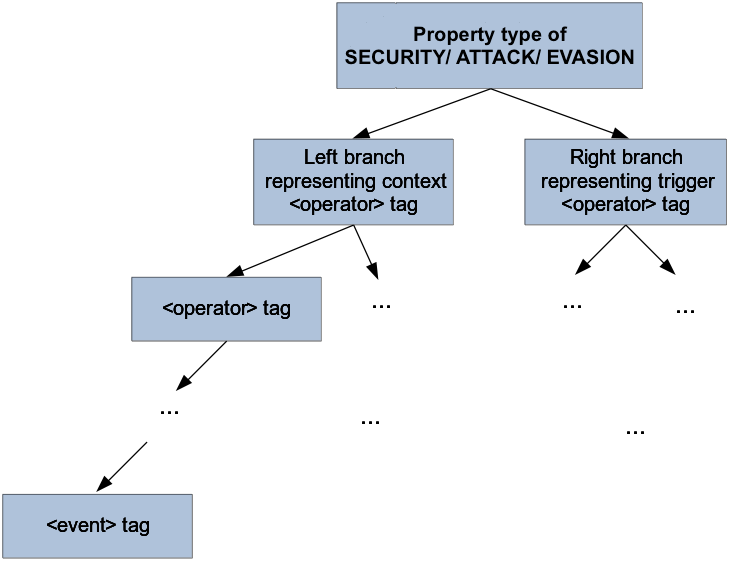
\includegraphics[width=4in]{img/rules.png}
\caption{MMT-Security property structure}\label{rules}
\end{figure}


\index{validation}\marginlabel{Property validation or violation:} The nodes of the property tree are: the property node (required),
operator nodes (optional) and event nodes (required). The property node
is forcibly the root node and the event nodes are forcibly leaf nodes.
In general, the left branch represents the context and the right branch represents
the trigger. This means that the property is found valid when the
trigger is found valid; and the trigger is checked only if the context
is valid. In other words:

\begin{itemize}
\item If the context is verified and the trigger is not, then a property
non-respect instance is detected.

\begin{itemize}
\item In the case of a \inlineCode{SECURITY} rule, this means that the context of the rule has
been found and, since the trigger was not, we conclude that the
\inlineCode{SECUIRTY} rule has been violated.
\item In the case of an \inlineCode{ATTACK} or \inlineCode{EVASION} rule,
this means that the context of an attack has occurred but the trace was
attack free because we did not detect the final trigger.
\end{itemize}
\item If the context and the trigger are verified, then a property
respect instance is detected.

\begin{itemize}
\item In the case of a \inlineCode{SECURITY} rule, this means that the context of the rule has
been found, as well as the trigger. We conclude that the
\inlineCode{SECURITY} rule has been respected.
\item In the case of an \inlineCode{ATTACK} or \inlineCode{EVASION} rule,
this means that the context of an attack has occurred, as well as the
trigger. We conclude that the behavioural attack/evasion has been detected.
\end{itemize}
\end{itemize}

To illustrate how a property is specified, a simplified instance of the Figure \ref{rules}) in XML gives :

\begin{lstlisting}[style = XML, title = General format of a property]
<property value="THEN" delay_units="s" delay_min="0+" delay_max="2" property_id="1" type_property="ATTACK" description="(description of attack)">
    <operator value="THEN" delay_max="1" >
    <event value="COMPUTE" event_id="1"
        description="(description of event 1)"
        boolean_expression="(Boolean expression allowing to detect event 1)"/>
    <event value="COMPUTE" event_id="2"
        description="(description of event 2)"
        boolean_expression="(Boolean expression allowing to detect event 2))"/>
    </operator>
    <event value="COMPUTE" event_id="3"
        description="(description of event 3)"
        boolean_expression="(Boolean expression allowing to detect event 3)"/>
</property>
\end{lstlisting}


\index{note}\note A context can occur before, at the same time or after a
trigger, depending on how the delays or counters attributes are defined (as explained in the next table \ref{prop_att}). To date, we have a library of MMT rules including the following types: 
\begin{itemize}
\item{Uni-packet rules: The events will be verified on the same packet, i.e., the extracted meta-data of one packet satisfy both the context and the trigger conditions.}
\item{Multi-packet, Uni-session rules: The events will be verified in multiple packets but belonging to the same session. This means that the source and destination IP addresses and ports correspond to the same session.}
\item{Multi-session, Uni-probe rules: The events will be verified in multiple packets in multiple sessions based on the reports coming from one single MMT-Probe.}
\item{Multi-session, Multi-probe rules: The events will be verified in multiple packets in multiple sessions based on the reports coming from several MMT-Probes.}
\end{itemize}

\index{propatt}\marginlabel{Property attributes:} The \inlineCode{<property>} tag
contains several attributes, some required, some optional:

\begin{table}[H]
\tablecaption{ Property tag attributes}\label{prop_att}
    \begin{adjustwidth}{-2in}{-.5in}
        \begin{center}
\begin{supertabular}{|m{1.0281599in}|m{1.0281599in}|m{1.0281599in}|m{3.44206in}|}
\hline
\rowcolor{Gray}
 Attribute &
Accepted values &
Req./opt., default value &
Description
\\\hline
property\_id &
Integer &
required &
Property id number, should go from 1 to n where n is the total number of
properties in the XML file. In one or different XML files, two different properties must have two different \inlineCode{property\_id}\\\hline
value &
\inlineCode{"THEN"}%, \inlineCode{"BEFORE"} 
&
required &
A property is a tree and each node can have one or more branches. The
{\textless}property{\textgreater} tag here represents the root of a
tree that can have 2 branches: the context and the trigger.

The value attribute indicates that the left
branch representing the context needs to be valid before, after or at the same time we check the
right branch representing the trigger, depending on the delays defined for the node.
\\\hline
type\_property &
\inlineCode{"ATTACK"},
\inlineCode{"EVASION"},
\inlineCode{"SECURITY"}&
required &
Indicates that the property specifies a potential attack/evasion (or abnormal
behaviour) or that the property specifies a security rule that needs to
be respected.\\\hline
\inlineCode{delay\_min} &
Integer &
optional, default value 0 &
Defines the validity period ([delay\_min, delay\_max]) of the left branch
(e.g. context). 

If we have [a,b] with a=b=0 then the left branch needs to occur in the
same time as the right branch. 

If we have a{\textless}b{\textless}=0 then the right branch needs to
have occurred in the past time interval with respect to the left
branch. 

If we have 0{\textless}=a{\textless}b then the right branch needs to
occur in the future with respect to the left branch. 

If the time runs out before detecting the events concerned then we are
in a TIMEOUT condition, i.e., the context occurs but the trigger never arrived in the specified time interval. This would mean that the property failed.  
Note that in the case that an event should not occur during a certain time interval, we refer to it as TIMEIN instead of TIMEOUT.
The default unit of time used is the second but this can be changed using the attribute delay\_units.
\\\hhline{---~}
delay\_max &
Integer &
optional, default value 0 &
For delay\_min, a + sign before the value (e.g.,  {\textquotedblleft}+0{\textquotedblright}) means strictly greater than the value and for delay\_max a - sign means less than.
\\\hline
delay\_units &
Integer &
optional, default value is {\textquotedblleft}s{\textquotedblright} (seconds) &
Defines the time units used in delay\_min and delay\_max attributes. If default value is not wished then this has to be defined before these two attributes. Possible values are Y,M,D,H,m,s(default),ms or mms.
\\\hline
counter\_max (under development)&
Integer &
optional, default value 0 &
Similar to [delay\_min, delay\_max] we can define [counter\_min,
counter\_max] where the unit is the number of packets analysed. 

If the count runs out before detecting the events concerned, then we are
in, respectively, a COUNTIN or COUNTOUT condition.
\\\hhline{---~}
counter\_min (under development)&
Integer &
optional, default value 0 &
\\\hline
description &
String &
required &
The text that clearly explains what the property is about.\\
\hline
\end{supertabular}
        \end{center}
    \end{adjustwidth}
\end{table}


\begin{table}[H]
\tablecaption{ Property tag attributes (cont.)}\label{prop_attb}
    \begin{adjustwidth}{-2in}{-.5in} 
        \begin{center}
\begin{supertabular}{|m{1.0281599in}|m{1.0281599in}|m{1.0281599in}|m{3.44206in}|}
\hline
\rowcolor{Gray}
 Attribute &
 Accepted values &
 Req./Opt., default value &
 Description
\\\hline
if\_satisfied &
String &
optional &
Defines what action should be performed if the property is satisfied. 
The string gives the name of the function that should be executed (see Reactive Functions~\ref{reactive_functions}).
%\\\hhline{---~}
%if\_not\_satisfied &
%String &
%optional &
\\\hline
%keep\_state &
%One or more event\_id{\textquotedblright}s separated by commas &
%optional &
%Allows indicating what event states should be kept. This is used when a property, for which the context becomes valid, should be able to detect all the triggers that occur in the defined time interval and not be {\textquotedblleft}consumed{\textquotedblright} by the first one.
%\\\hline
\end{supertabular}
        \end{center}
    \end{adjustwidth}
\end{table}



\index{opatt}\marginlabel{Operator attributes:} The {\textless} operator{\textgreater} tag in a property contains
several attributes, some required, some optional:


\begin{table}[H]
\tablecaption{ Operator tag attributes}\label{op_att}
    \begin{adjustwidth}{-2in}{-.5in} 
        \begin{center}
\begin{supertabular}{|m{1.0281599in}|m{1.0281599in}|m{1.0281599in}|m{3.44206in}|}
\hline
\rowcolor{Gray}
 Attribute &
 Accepted values &
 Req./Opt., default value &
 Description
\\\hline
value &
\inlineCode{"THEN"},
\inlineCode{"OR"},
\inlineCode{"AND"},
\inlineCode{"NOT"} &
required &
Operators are used to combine different events and build complex events.
{\textquotedblleft}THEN{\textquotedblright} operator is used to
describe ordered events, {\textquotedblleft}AND{\textquotedblright}
operator is used to describe two events without any order and
{\textquotedblleft}OR{\textquotedblright} operator is used to describe
the occurrence of a least one of the events. {\textquotedblleft}NOT{\textquotedblright} negates the underlying sub-tree.\\\hline
description &
String &
optional &
Gives the text that clearly explains what the complex event is
about.\\\hline
delay\_min &
Integer &
optional, default value 0 &
Same as for the {\textless}property{\textgreater} tag. Note that these
attributes are not to be used for the
{\textquotedblleft}OR{\textquotedblright} and {\textquotedblleft}NOT{\textquotedblright} operators.
\\\hhline{---~}
delay\_max &
Integer &
optional, default value 0 &
\\\hhline{---~}
counter\_max &
Integer &
optional, default value 0 &
\\\hhline{---~}
counter\_min &
Integer &
optional, default value 0 &
\\\hline
repeat\_times (under development) &
Integer &
optional, default value 1 &
Allows detecting the repetition of a complex event occurrence a number of times.\\\hline
\end{supertabular}
        \end{center}
    \end{adjustwidth}
\end{table}

\index{evatt}\marginlabel{Event attributes:} Properties indicate the sequence of events that need to be observed. Events
indicate the conditions that need to be verified on a packet or a set of packets for the event to hold. The {\textless}event{\textgreater} tag in a property
contains several attributes, some required, some optional:


\begin{table}[H]
\tablecaption{Event tag attributes}\label{ev_att}
    \begin{adjustwidth}{-2in}{-.5in} 
        \begin{center}
\begin{supertabular}{|m{1.3941599in}|m{1.0254599in}|m{1.0004599in}|m{3.10736in}|}
\hline
\rowcolor{Gray}
 Attribute &
 Accepted values &
 Req./Opt., default value &
 Description
\\\hline
event\_id &
Integer &
required &
This field allows identifying each event and starts from 1 to n where n is the total number of events in the current property.\\\hline
description &
String &
required &
Gives the text that clearly explains what the event is about.\\\hline
value &
\inlineCode{"COMPUTE"} &
required &
Means that the events need to resolve a Boolean expression that is equal
to \inlineCode{true} or
\inlineCode{false} depending on the
attributes values\\\hline
boolean\_expression &
expression &
required &
A Boolean expression, similar to a Boolean expression in the C language
(explained in the following paragraph).\\\hline
\end{supertabular}
        \end{center}
    \end{adjustwidth}
\end{table}


\index{bool}\marginlabel{Boolean expressions:} The \inlineCode{boolean\_expression} is a logical combination of
{\textquotedblleft}{\textless}protocol
name{\textgreater}.{\textless}field
name{\textgreater}{\textquotedblright} and
{\textquotedblleft}{\textless}number{\textgreater}{\textquotedblright}
with the following operators:
{\textquotedblleft}\&\&{\textquotedblright},
{\textquotedblleft}{\textbar}{\textbar}{\textquotedblright},
{\textquotedblleft}{\textgreater}{\textquotedblright},
{\textquotedblleft}{\textgreater}={\textquotedblright},
{\textquotedblleft}{\textless}{\textquotedblright},
{\textquotedblleft}{\textless}={\textquotedblright},
{\textquotedblleft}=={\textquotedblright},
{\textquotedblleft}!={\textquotedblright},
{\textquotedblleft}+{\textquotedblright},
{\textquotedblleft}-{\textquotedblleft},
{\textquotedblleft}/{\textquotedblright},
{\textquotedblleft}*{\textquotedblright}. Blanks and tabs are ignored.
Note that the {\textquotedblleft}\&\&{\textquotedblright} operator
needs to be written in XML as
{\textquotedblleft}\&amp;\&amp;{\textquotedblright}, 
{\textquotedblleft}{\textless}{\textquotedblright} 
needs to be written as
{\textquotedblleft}\&lt;{\textquotedblright}, etc.


A simple \inlineCode{boolean\_expression} can be of the form: 

\begin{center}
\inlineCode{  (<expression> <operator> <expression>) }
\end{center}

in which, \inlineCode{<expression>} is one of the followings:

\begin{itemize}
    \item \inlineCode{<protocol\_name>.<attribute\_name>}
    \item \inlineCode{<protocol\_name>.<attribute\_name>.<event\_id>}
    \item \inlineCode{<numeric\_value>}
    \item \inlineCode{<string\_value>}
    \item \inlineCode{true}
    \item \inlineCode{false}
    \item embedded function
\end{itemize}


The Boolean expressions must respect some syntax rules:

\begin{itemize}
\item The building bloc needs to start with a
\textQuote{(} and end with a \textQuote{)}. Note that to avoid any ambiguities the quotes should explicitly define how the expression is to be resolved, e.g, A \&\& B {\textbar}{\textbar} C should be written as ((A \&\& B) {\textbar}{\textbar} C) or (A \&\& (B {\textbar}{\textbar} C)).
\item An attribute needs to be identified with its \inlineCode{protocol\_name} and
its \inlineCode{attribute\_name} separated by a dot
\textQuote{.}.
\item If the attribute refers to an attribute value from another event,
then the name needs to be followed by a second
\textQuote{.} and the \inlineCode{event\_id} number of
the event concerned. For instance we can have:

\begin{itemize}
\item \inlineCode{(arp.ar\_op == 0)}
means that the field \inlineCode{arp.ar\_op} should be equal to zero.
\item \inlineCode{(arp.ar\_op == arp.ar\_op.1)} means that the field  
\inlineCode{arp.ar\_op} should be equal to the field \inlineCode{arp.ar\_op} of the event in the same rule with the \inlineCode{event\_id} equal to 1.
\end{itemize}
\end{itemize}


\index{exbool}\marginlabel{Example of a Boolean expression:} For example; the following expression means that the event is valid if
the packet received corresponds to the ARP protocol;
the \inlineCode{ar\_op} is 2; \inlineCode{ar\_sip} is the same as \inlineCode{ar\_tip}
of an event 1; and, \inlineCode{ar\_sha} is different with \inlineCode{ar\_sha} of event 2. Where events 1 and 2 occurred before or will occur after depending on the order that the events should occur (defined by the time intervals specified).

% "((((arp.ar_op == 2)&amp;&amp;(arp.ar_sip == arp.ar_tip.1))&amp;&amp;(arp.ar_sha != arp.ar_sha.2)) &amp;&amp; (ethernet.packet_count != 0))"
\inlineCode{"(((arp.ar\_op == 2)\&amp;\&amp;(arp.ar\_sip == arp.ar\_tip.1)) \&amp;\&amp;(arp.ar\_sha != arp.ar\_sha.2))"}

% \begin{table}[H]
%     \begin{adjustwidth}{-1in}{-.5in} 
% \ \ \ \ \ \ \ \ \ \ \ \ \ \ \ \ \ \ \ \ \ \ \ boolean\_expression={\textquotedbl}(((ARP.OPCODE == 2)\&amp;\&amp;

% \ \ \ \ \ \ \ \ \ \ \ \ \ \ \ \ \ \ \ \ \ \ \ (ARP.SRC\_PROTO == ARP.DST\_PROTO.1))\&amp;\&amp;

% \ \ \ \ \ \ \ \ \ \ \ \ \ \ \ \ \ \ \ \ \ \ \ (ARP.SRC\_HARD == ARP.SRC\_HARD.2)){\textquotedbl}
%     \end{adjustwidth}
% \end{table}

The following table gives a more detailed explanation about the
information that is used in the Boolean expression:


\begin{table}[H]
\tablecaption{ Boolean expressions}\label{bool}
    \begin{adjustwidth}{-2in}{-.5in} 
        \begin{center}
\begin{supertabular}{|m{1.0in}|m{1.0in}|m{4.52616in}|}
\hline
\rowcolor{Gray}
 Name &
 Type &
 Description
\\\hline
protocol\_name &
String &
Indicates the protocol of the packet that we need to inspect.\\\hline
attribute\_name &
String &
Indicates the field of the protocol that we will use for verifying a
condition in the event.\\\hline

numeric\_value &
Integer &
Gives the value that will be used to compare with the packet field
value. Note that the
\inlineCode{protocol\_name} and the
\inlineCode{attribute\_name} allow uniquely
identifying the type of value a field contains (e.g. number, IP
address, MAC address in binary format).

Two specific constants, \inlineCode{true} and \inlineCode{false}, represent respectively a non-zero and zero number.
\\\hline

string\_value & 
String &

Gives a chain of characters, enclosed by ' and ', \eg,
\inlineCode{'GET'}
\\\hline

reference &
Integer &
Indicates that we are to use the data obtained for the field from an
event that occurred before (a previously received packet that validated
the previous event). The name is a number that clearly identifies the
event and needs to be exactly the same as the value given in the
\inlineCode{event\_id} attribute of the corresponding {\textless}event{\textgreater}
tag. Note that one should refer to events that occurred beforehand in the property.\\\hline
\end{supertabular}
        \end{center}
    \end{adjustwidth}
\end{table}

\index{extensions}\marginlabel{Extensions:} Embedded functions can be used to extend the elements used in the Boolean expressions (see section~\ref{Embedded}).

\index{compilation}\marginlabel{Property compilation:} After creating the XML properties, we need to compile them by using the executable \inlineCode{compile\_rule}: 
\begin{lstlisting}[style=BASH]
./compile_rule <rule_name>.so <property>.xml
\end{lstlisting} 
%****************************************************


%****************************************************

\subsection{Embedded Functions}
\label{Embedded}
Embedded functions are functions that allow implementing calculations that are too complicated to define using only classical operators on fields in the Boolean expressions of security properties. One can use existing embedded functions or implement a new function. In both cases, they can be used in the Boolean expressions by using the syntax:

\#<name\_of\_function>(<list of parameters>)

For instance:

\inlineCode{(\#em\_is\_search\_engine( http.user\_agent ) == true)}

where \inlineCode{http} is the protocol name and \inlineCode{user\_agent} is the attribute name (i.e., packet meta-data).

\marginlabel{Implement new\\Embedded Functions:}
The embedded functions must respect the C syntax and are used in Boolean expressions using the syntax described above.
Embedded functions are implemented inside \inlineCode{<embedded\_functions>} tag of the XML rule files and will be compiled together with the rules. 
The input parameters are either of the type \inlineCode{const char * } or \inlineCode{int val}. 
For instance, the \inlineCode{em\_is\_search\_engine} above could be implemented as follows:

\begin{lstlisting}[style=Cpp]
<embedded_functions><![CDATA[
//code C
static inline bool em_is_search_engine(const char *agent){
    if( strstr( agent, "google" ) != NULL )
        return true;
    if( strstr( agent, "bing" ) != NULL )
        return true;
    return false;
}]]></embedded_functions>
\end{lstlisting}

\note: The function name should be prefixed by \inlineCode{em\_} to avoid any confusion with other functions in the system.

One can also implement code into 2 other functions to initialize and free common resource:
\begin{itemize}
    \item \inlineCode{void on\_load()\{ ... \}} is called when the rules inside the XML file being loaded into MMT-Security

    \item \inlineCode{void on\_unload()\{ ... \}} is called when exiting MMT-Security
\end{itemize}


\marginlabel{Pre-implemented\\Embedded Functions:} There exist several embedded functions that have been implemented inside MMT-Security.

\begin{enumerate}
    \item \inlineCode{is\_exist( proto.att )} checks whether an event has an attribute of a protocol, \eg, \inlineCode{is\_exist( http.method )} will return \inlineCode{true} if the current event contains protocol HTTP and attribute \inlineCode{method} has a non-null value, otherwise it will return \inlineCode{false}.

    Normally MMT-Security has a filter that allows an event in a rule to be verified only if any proto.att used in its boolean expression contains value. If one of them has not, the rule will not be verified. This allows to reduce number of verification of boolean expression, thus increases the performance.

    For example, given an event having the following boolean expression:
    
    \begin{center}
    \inlineCode{((ip.src != ip.dst) \&\& (\#em\_check\_URI(http.uri) == 1))}
    \end{center}

    This expression is verified only if \inlineCode{ip.src} and \inlineCode{ip.dst} and \inlineCode{http.uri} are not null, hence only HTTP packets are verified (it does not verify every IP packets).

    However, if one use the following expression, that is totally having the same meaning with the previous one:

    \begin{center}
        \inlineCode{((ip.src != ip.dst) \&\& ((#is\_exist(http.uri) == true ) \&\& (\#em\_check\_URI(http.uri) == 1)))}
    \end{center}
    
    MMT-Security need to verify the expression against any IP packet as the \inlineCode{is\_exist} function tell MMT to exclude \inlineCode{http.uri} from its filter.


    \item \inlineCode{is\_empty( proto.att )}, e.g., \inlineCode{is\_empty(http.uri)} checks whether the string value is empty, i.e., its length is zero.

    \item User can use {\em any standard C functions} as embedded function, \eg, \inlineCode{(\#strstr( http.user\_agent, 'robot') != 0)} to check if \inlineCode{http.user\_agent} contains a sub-string \inlineCode{"robot"}.
    
    
    \note Before using a C function, the library containing that function need to be included.
    The following libraries have been pre-included:

    \begin{lstlisting}[style=Cpp]
#include <string.h>
#include <stdio.h>
#include <stdlib.h>
#include "mmt_lib.h"
#include "pre_embedded_functions.h"
    \end{lstlisting}
    
    Thus when using a function that does not defined inside these libraries, one need to include its library. For example:
\begin{lstlisting}[style=Cpp]
<embedded_functions><![CDATA[
#include <math.h>

static inline bool function em_check( double port ){
    double x = sqrt( port );
    ...
}
]]></embedded_functions>
\end{lstlisting}

\end{enumerate}

\marginlabel{Reactive Functions:}\label{reactive_functions}
Reactive functions allow user perform some action when a rule is satisfied.
The functions will be called each time their rules are satisfied. 
When a security and attack rules are satisfied, they will give \inlineCode{not\_respected} and \inlineCode{detected} verdicts respectively.

To implement and use a reactive function, one need to

\begin{enumerate}
    \item 
implement a C function inside \inlineCode{<embedded\_functions>} tag.
The function has the following format:

\begin{lstlisting}[style=Cpp]
typedef void (*mmt_rule_satisfied_callback)(
  const rule_t *rule,//rule being validated
  int verdict,       //DETECTED, NOT_RESPECTED
  uint64_t timestamp,//moment (by time) the rule is validated
  uint64_t counter,  //moment (by order of message) the rule is validated
  const mmt_array_t * const trace  //messages that validate the rule
);
\end{lstlisting}

\item put the function name in attribute \inlineCode{if\_satisfied} of the rule you want to react. For example: \inlineCode{if\_satisfied="em\_print\_out"}

\begin{lstlisting}[style=Cpp]
<beginning>
<embedded_functions><![CDATA[
static void em_print_out( const rule_info_t *rule, int verdict, uint64_t timestamp, uint64_t counter, const mmt_array_t * const trace ){
   const char* trace_str = mmt_convert_execution_trace_to_json_string( trace, rule );
   printf( "detect rule %d\n%s\n", rule->id, trace_str );
}]]></embedded_functions>

<property value="THEN" delay_units="s" delay_max="0" property_id="10" type_property="EVASION" 
    description="HTTP using a port different from 80 and 8080." if_satisfied="em_print_out">
    <event value="COMPUTE" event_id="1" 
        description="a port different from 80 and 8080"
           boolean_expression="((http.method != '')&amp;&amp;((tcp.dest_port != 80)&amp;&amp;(tcp.dest_port != 8080)))"/>
    <event value="COMPUTE" event_id="2" 
           description="HTTP packet"
           boolean_expression="(ip.src != ip.dst)"/>
</property>
</beginning>
\end{lstlisting}

\end{enumerate}

\marginlabel{High Performance Rules:}
To write a rule having a high performance, one need to:

\begin{itemize}
    \item 
use only the proto.att in boolean expression when need

Please refer to the usage of function \inlineCode{is\_exist} to get an example.

\item Use explicitly the following tcp flags to filter out unwanted verification: tcp.fin, tcp.syn, tcp.rst, tcp.psh, tcp.ack, tcp.urg, tcp.ece, tcp.cwr.

For example, the 2 following boolean expressions have the same meaning:

\inlineCode{(tcp.flags == 4)} and 
\inlineCode{((tcp.flags == 4) && (tcp.rst == 1))}

They both return true when only RST flag of a TCP packet is on, but the latter is better as MMT verifies its rule only when tcp.flags and tcp.rst are not zero. Usually less than about 1\% packets having \inlineCode{tcp.rst != 0}, consequently the rule using the second expression will be verified against only 1\% packets.

\item reduce \inlineCode{delay\_max} of a rule to a suitable value

When having a higher value of \inlineCode{delay\_max} MMT-Security creates more rule instances to correlate different events of different packets. When \inlineCode{delay\_max} is zero, the rule is call simple rule, MMT-Security verifies the rule and gives verdict immediately without creating any rule instances. A simple rule is verified much faster than a complex one that has non-zero \inlineCode{delay\_max}.

\recommend MMT-Security can verify 12400 simple rules or 600 complex rules at 10Gbps.

\item optimize implementation of embedded functions

The embedded functions are called each time their boolean expressions are verified. Consequently, rather than initialize something, for example, connection to database, inside these functions, one can do such a task, only once, inside function \inlineCode{on\_load} then store the connection into a static local variable that will be used inside the embedded functions.

\item always use embedded function with \inlineCode{static inline} keyword

For more information about advantage of inline, please refer to document of gcc: {\em An Inline Function is As Fast As a Macro}.
\end{itemize}
%****************************************************


%****************************************************

\subsection{Example}
\subsubsection{Property without Embedded Functions: ARP Spoofing Example}
\label{arp_example}
In order to provide a complete but easy to understand example, the detection of ARP spoofing is presented here in detail. 

\index{arp}\marginlabel{ARP spoofing:} Address Resolution Protocol (ARP) is a telecommunications protocol used for resolution of network layer addresses into link layer addresses, a critical function in multiple-access networks. ARP was defined by RFC 826 in 1982\footnote{\url{https://en.wikipedia.org/wiki/Address_Resolution_Protocol}}. 
ARP spoofing\footnote{\url{https://en.wikipedia.org/wiki/ARP_spoofing}}(RFC5227\footnote{\url{http://www.networksorcery.com/enp/rfc/rfc5227.txt}}) is a technique used to attack a local-area network (LAN). ARP spoofing may allow an attacker to intercept data frames on a LAN, modify the traffic, or stop the traffic altogether. Figure~\ref{arp} represents an attack by a device using MAC address MAC3 (in red).

\begin{figure}[H]
\centering
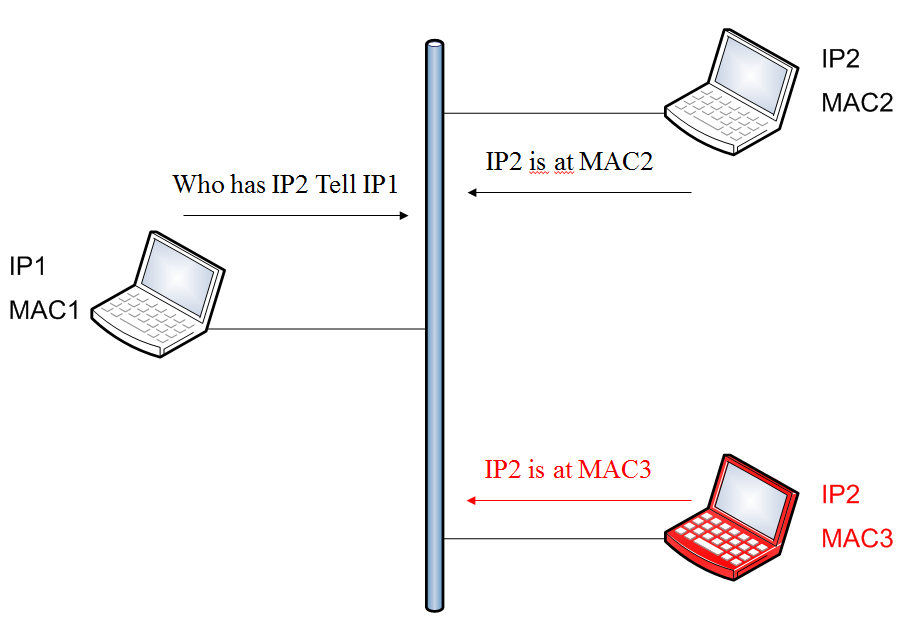
\includegraphics[width=4in]{img/arp_example.png}
\caption{ARP spoofing}\label{arp}
\end{figure}

\index{model}\marginlabel{Attack model:} Following an ARP request (\textit{who has}), a node receives more than one reply with different MAC addresses. This could mean that an IP duplication has been detected that could potentially be an ARP spoofing attack.

This attack behaviour can be specified as follows:

\begin{displaymath} 
 (e\textsubscript{1} ; e\textsubscript{2})\textsubscript{0,4}\hspace{2 mm} AFTER \textsubscript{0,10}\hspace{2 mm} e\textsubscript{3}
\end{displaymath}
Where:


\begin{itemize}
\item \textbf{Event 1} (e\textsubscript{1}): reception of ARP request message
\item \textbf{Event 2} (e\textsubscript{2}): reception of ARP reply message (src MAC2)
\item \textbf{Event 3} (e\textsubscript{3}): reception of ARP reply message with (scr MAC3) != (src MAC2)
\item \textbf{AFTER\textsubscript{0,4}} is an operator indicating that event e\textsubscript{3} occurs after the occurrence of the sequence of events e\textsubscript{1} ; e\textsubscript{2} with a time interval that represents the interval defined in RFC5227 between conflicting ARPs below which a host must not attempt to defend its address. This interval could be reduced or increased to detect spoofing attempts and avoid to many verdicts that are false positives.
\end{itemize}

\bigskip

This security attack is specified by MMT-Security rule as the following:
\lstinputlisting[style=XML]{img/4.arp.xml}

\subsubsection{Property with an Embedded Function: NFS Example}
This property aims to detect the occurrence of the event: "NFS Client uploads a file synchronized to another server" (Fig.~\ref{nfs_upload}). This action can violate the privacy of the data within an organization\rq s network. 
\begin{figure}[H]
\centering
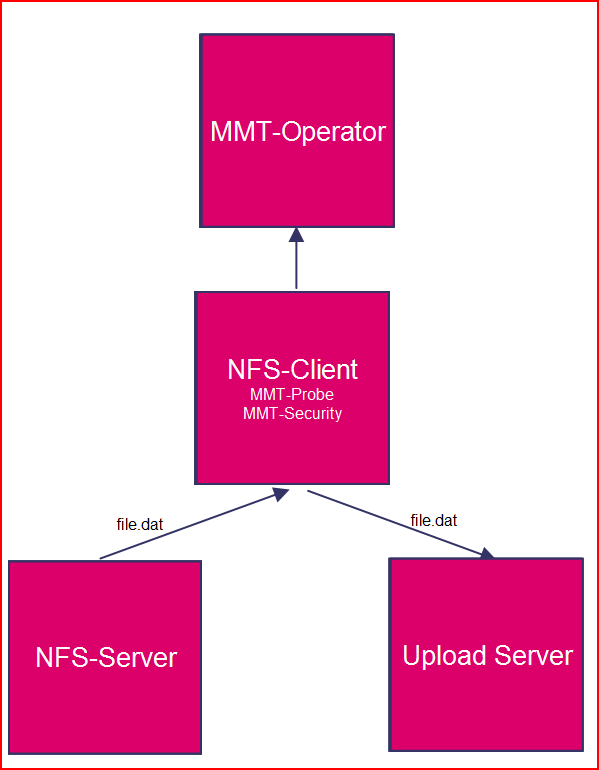
\includegraphics[width=3in]{img/nfs.PNG}
\caption{Upload a file synchronized from NFS Server to another server}
\label{nfs_upload}
\end{figure}

\marginlabel{Using a pre-implemented standard C function:} Suppose that we have one MMT-Probe that assesses NFS traffic as well as HTTP traffic. The attack behaviour can be specified by an MMT rule as follows:
\begin{displaymath} 
(e\textsubscript{1} ; e\textsubscript{2})\textsubscript{0,20}
\end{displaymath}
\lstinputlisting[style=XML]{img/nfs_upload.xml}

Where: 
\begin{itemize}
\item \textbf{Event 1} (e\textsubscript{1}): The reception of an NFS synchronization packet and extraction of the file\rq s name.
\item \textbf{Event 2} (e\textsubscript{2}): The reception of an HTTP packet with the file\rq s name in the payload (verified by the function \inlineCode{\#strstr(tcp.p\_payload, nfs.file\_name.1)}).  
\end{itemize}


\marginlabel{Using a new embedded function:} Suppose that we have two MMT-Probes: One verifies NFS traffic and sends reports to the REDIS bus. The other, analyzes HTTP traffic and uses an Embedded Function to also report to the REDIS bus. The attack behaviour can be specified in an MMT rule as follows:
\begin{displaymath} 
(e\textsubscript{1} ; e\textsubscript{2})\textsubscript{0,0}
\end{displaymath}

\lstinputlisting[style=Cpp]{img/nfs_redis.xml}

Where:
\begin{itemize}
\item \textbf{Event 1} (e\textsubscript{1}): The reception of an HTTP packet with payload length greater than 0.
\item \textbf{Event 2} (e\textsubscript{2}): The embedded function, \inlineCode{em\_check\_nfs\_redis}, is called to:
\begin{itemize}
\item Get the names of all the files synchronized by the NFS Server. These reports are generated by another MMT-Probe and stored in the REDIS bus.   
\item Verify if the name of the file, \textit{file name}, is found in the packet payload. 
\end{itemize}
\end{itemize}



%****************************************************


%****************************************************

\subsection{Other Case Studies}
\label{Other}


Applying MMT-Security to a particular industrial scenario usually involves the following steps: 
\begin{enumerate}
\item
Develop any plugins needed to parse the data to be analysed. Note that parsers for most Internet protocols and applications are already available.
\item
Develop a {\textquotedbl}main.c{\textquotedbl} that will use the libraries to capture and analyse the data.
\item
Define a set of properties that specify the analysis to be performed. 
\end{enumerate}

The tool has been applied or is being applied to several industrial scenarios, such as:
\begin{itemize}
\item Generating broadband reporting for 4G mobile networks (for an equipment manufacturer);
\item Capturing information useful for detecting botnets and other cyber attacks (\url{http://www.acdc-project.eu/} and \url{https://sissden.eu/});
\item Detecting malicious nodes in an ad-hoc network (\url{http://projects.celtic-initiative.org/SAN/});
\item Estimating user Quality of Experience (QoE) of video flows (for an equipment manufacturer);
\item Analysing and fine tuning of delay tolerant networks;
\item Detecting and mitigating attacks in radio protocol communications, Near Field Communication ecosystems and vehicular communications (\url{http://www.itea2-diamonds.org/index.html});
\item Monitoring secure interoperability (\url{http://inter-trust.eu/});
\item Performance analysis for web sites (\url{http://genibeans.com/cgi-bin/twiki/view/Pimi/WebHome/} and \url{http://swept.eu/});
\item Monitoring function for security and performance of Software Defined 5G Mobile Networks, Datacenters, Critical Infrastructures, Cloud infrastructures and services, Cyber-Physical Systems;
\end{itemize}

%ISER, MEVICO/SIGMONA, INQPSIS/NOTTS, PIMI 

%****************************************************

\subsection{Compile MMT-Security Rules}

MMT-Security rules are specified in plain text following an XML format. The rules need to be compiled into a dynamic C library used by MMT.

The compiled rules must put in either \path{./rules} or \paht{/opt/mmt/security/rules}.
The former has higher priority and only one of them will be taken into account by MMT-Security.
Specifically, if MMT-Security found \path{./rules} folder in the current folder executing, it will use the rules inside this folder and
it does not take into account the rules in \path{/opt/mmt/security/rules}.

\marginlabel{Compile rules:}
MMT provides a tool to compile the rules: \path{/opt/mmt/security/bin/compile_rule}. To execute it do:

\begin{lstlisting}[style=BASH]
./compile_rule output_file property_file [-c] [gcc param]
\end{lstlisting}

where:

\begin{enumerate}
\item \inlineCode{output\_file}: is the path of file containing the result that can be either a .c file or .so file.
\item \inlineCode{property\_file}: is the path where the property file can be found.
\item optional parameters: 
    \begin{itemize}
    \item \inlineCode{-c}: will generate only the C code. This option allows manually modifying the generated code before compiling it. 
    After generating the C code, the tool prints out the command that needs to be executed for compiling it.
    
    \item \inlineCode{gcc param}: used to generate the C code, and compile it to obtain the .so file.
                   These parameters will be directly transmitted to the gcc compiler, for example, \inlineCode{"-I/home/tata/include -lmath"}
    \end{itemize}
\end{enumerate}

For example, the following command compiles the rule detecting arp spoofing presented above:

\begin{lstlisting}[style=BASH]
./compile_rule /opt/mmt/security/rules/arp.so arp.xml
\end{lstlisting}

\marginlabel{Obtain information from\\ the compiled rules:} To get some basic information about the compiled rules (such as, ID, description) MMT provides a tool: \path{/opt/mmt/security/bin/rule_info}.

\begin{itemize}
\item By default, the tool will print out the information on all rules located in \path{/opt/mmt/security/rules/}, for instance:

\begin{lstlisting}[style=CONFIG]
/opt/mmt/security/bin/rule_info 
Found 35 rules.
1 - Rule id: 1
	- type            : attack
	- events_count    : 4
	- variables_count : 5
	- variables       : ip.dst (178.13), ip.src (178.12), tcp.dest_port (354.2), tcp.flags (354.6), tcp.src_port (354.1)
	- description     : Several attempts to connect via ssh (brute force attack). Source address is either infected machine or attacker (no spoofing is possible).
	- if_satisfied    : (null)
	- if_not_satisfied: (null)
	- create_instance : 0x7fad94d0be80
	- hash_message    : 0x7fad94d0bd50
	- version         : 1.1.2 (67fa423 - 2017-5-19 18:14:31), dpi version 1.6.8.0 (b3e727b)
2 - Rule id: 10
	- type            : evasion
	- events_count    : 2
	...
...
\end{lstlisting}

\item The tool can also be used to inspect a specific compiled rule by giving the rule path as parameter, for instance:

\begin{lstlisting}
./rule_info /opt/mmt/security/rules/4.arp.so 
Found 1 rule.
1 - Rule id: 4
	- type            : attack
	- events_count    : 3
	- variables_count : 7
	- variables       : arp.ar_op (30.5), arp.ar_sha (30.6), arp.ar_sip (30.7), arp.ar_tip (30.9), ethernet.dst (99.2), ethernet.packet_count (99.4099), ethernet.src (99.3)
	- description     : IPv4 address conflict detection (RFC5227). Possible arp poisoning.
	- if_satisfied    : (null)
	- if_not_satisfied: (null)
	- create_instance : 0x7f5063e7be70
	- hash_message    : 0x7f5063e7bcd0
	- version         : 1.1.2 (67fa423 - 2017-5-19 18:14:34), dpi version 1.6.8.0 (b3e727b)
\end{lstlisting}
\end{itemize}
%%%%%%%%%%%%%%%%%%%%%%%%%%%%%%%%%%%%%%%%%%%%%%%%%%%%%%%%%%%%%%%%%%%%%%
